%This chapter contains the background knowledge to optimise the understanding of patellofemoral pain and deep learning. The chapter is divided into the following sections: Anatomy of the knee, Pain, Pain mapping and Knee regions. Futhermore, machine learning and deep learning are specified.

%"Introduction to the chapter, shouldn’t be a list of what the chapter contains. It should be more what you gain by reading the chapter"

This chapter presents the background knowledge that optimizes the understanding of essential topics in this project, such as patellofemoral pain and deep learning. Regarding patellofemoral pain it is relevant to get knowledge about the anatomy of the knee as well as pain and pain measurements if a deeper understanding of the syndrome is considered necessary.  Furthermore, the chapter is essential for getting a basic understanding of some properties and optimizers in the neural network models used in this project.


\section{Anatomy of the Knee}
The knee is the largest synovial joint in the body and consists of a hinge and a gliding joint. The hinge joint is placed between the lateral and medial femoral condyles and the lateral and medial tibial condyles. Between the patella and femur is the gliding joint formed. The structure of the knee is illustrated in figure \ref{fig:bonestruc}.\citep{Martini2012}

\begin{figure} [H]
\centering
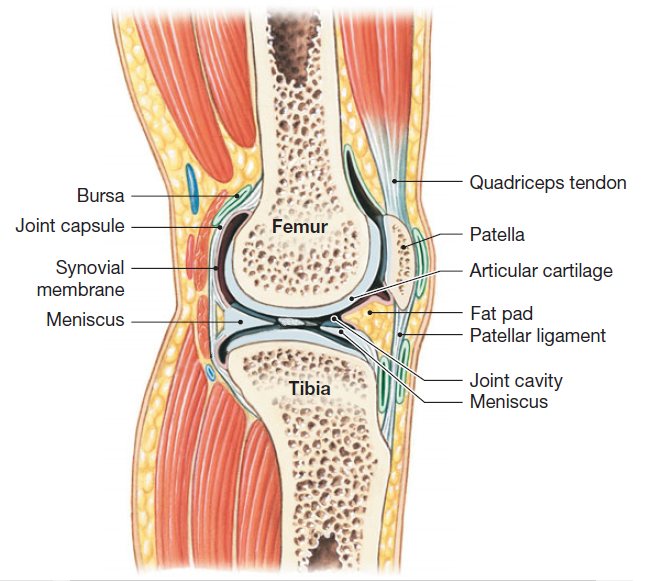
\includegraphics[width=0.7\textwidth]{figures/bonestruc}
\caption{The anatomy of the knee. Edited \citep{Martini2012}.}
\label{fig:bonestruc}
\end{figure}

\noindent
It is shown in figure \ref{fig:bonestruc} that the patella is a sesamoid bone. At birth the patella consists of cartilaginous and ossifies when the child’s extremities gets stronger, which typically proceeds between age two or three and the beginning of puberty. \\
\noindent
The patella is surrounded by the tendon of the quadriceps femoris. Quadriceps femoris is the muscles which controls the extending of the knee. The quadriceps tendon is combined to the surface anterior and superior of patella. Tibia is combined to the anterior and inferior surface of the patella by the patellar ligament. The bones, tibia and femur, are covered by articular cartilage with the purpose of protecting the bones from friction. The articular cartilage on the two bones are separated from one another by synovial membranes that contains synovial fluid, that further reduce the friction. The primary functions of the synovial fluid is to lubricate, distribution of nutrient and absorption of shock.\citep{Martini2012}\newline
\noindent
The fat pads and menisci are placed between the articular cartilages. The fat pads’ function is to protect the cartilage and fill out space as result of the joint cavity changes. The menisci stabilize the knee and acts like pads, that conform shape when femur moves. In addition to fat pads and menisci, the bursa acts as friction minimization between patella and tissues.\citep{Martini2012} \\
There are three separate articulations in the knee joint. The first is between the patella and the patellar surface of the femur and the rest are between the femoral and tibial condyles. Additionally, the knee consist of seven major ligaments that stabilize the knee joint, which are shown in figure \ref{fig:knee}.\citep{Martini2012}

\begin{figure} [H]
\centering
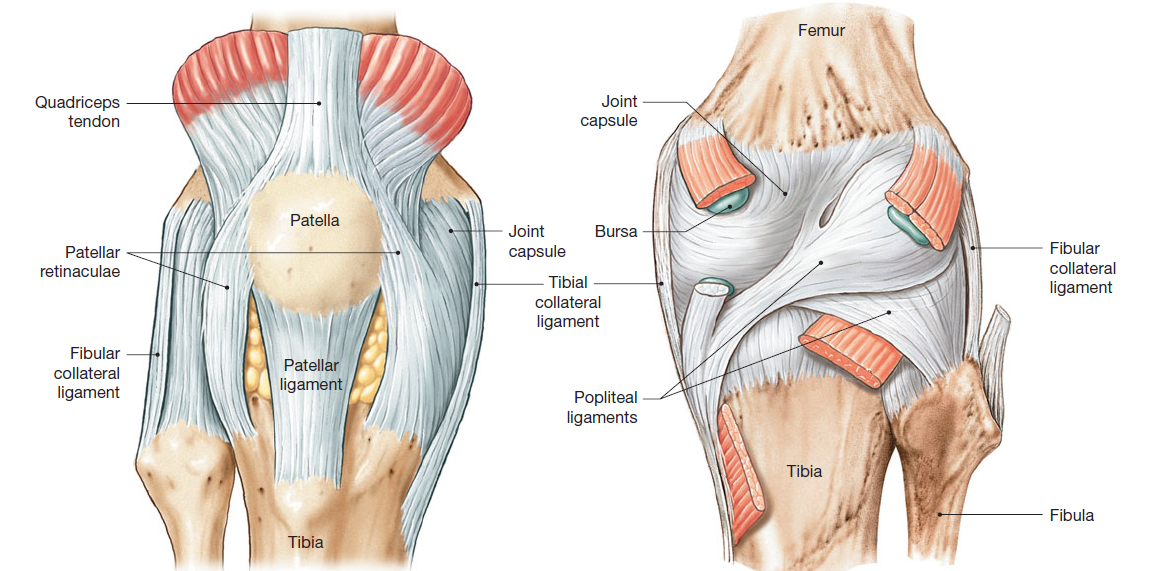
\includegraphics[width=1\textwidth]{figures/knee}
\caption{The anatomy of the knee with focus on the ligaments. Edited \citep{Martini2012}.}
\label{fig:knee}
\end{figure}

\noindent
The ligaments patellar retinaculae and patellar ligament support the anterior surface of the knee. When the knee is fully extended, the tibial and fibular collateral ligament are responsible for stabilizing the joint. Between femur and the two lower bones in the leg, tibia and fibula, is the location of the two popliteal ligaments, which stabilize the posterior surface of the joint. In addition to the visible ligaments in figure \ref{fig:knee} there are the anterior cruciate ligament (ACI) and posterior cruciate ligament (PCL) in the joint capsule. The two ligaments cross each other and are connected to the tibial and femoral condyles, which reduce the movement, anterior and posterior.\citep{Martini2012}\newline
\noindent


\section{Pain}
The International Association for the Study of Pain (IASP) has defined pain as being “an unpleasant sensory and emotional experience associated with actual or potential tissue damage or described in terms of such damage” \citep{IASP2012, Schmidt1989}.

\noindent
Humans are aware of the surroundings and threats to their bodies because of the pain. The pain indicates that there might be a risk for permanent damage on the body, which refrain humans from danger and therefore increases the chances of survival. 


\noindent
Pain can be either nociceptive or neuropathic. Nociceptive pain is associated with tissue damage. This type of pain is related to the nociceptors, which are receptors with a high threshold that when stimulated may give the perception of pain in tissues \citep{Schmidt2013}. Neuropathic pain occurs central from the nervous system. This pain can be caused by illness or physical damage.\citep{Schmidt2013} \\


\noindent
Furthermore, pain can be divided into three categories: acute pain (less than three months), persistent or chronic pain and cancer pain.\citep{Briggs2010} Additionally, the pain can be divided into qualities, which is shown in figure \ref{fig:qualities}. 

\begin{figure} [H]
\centering
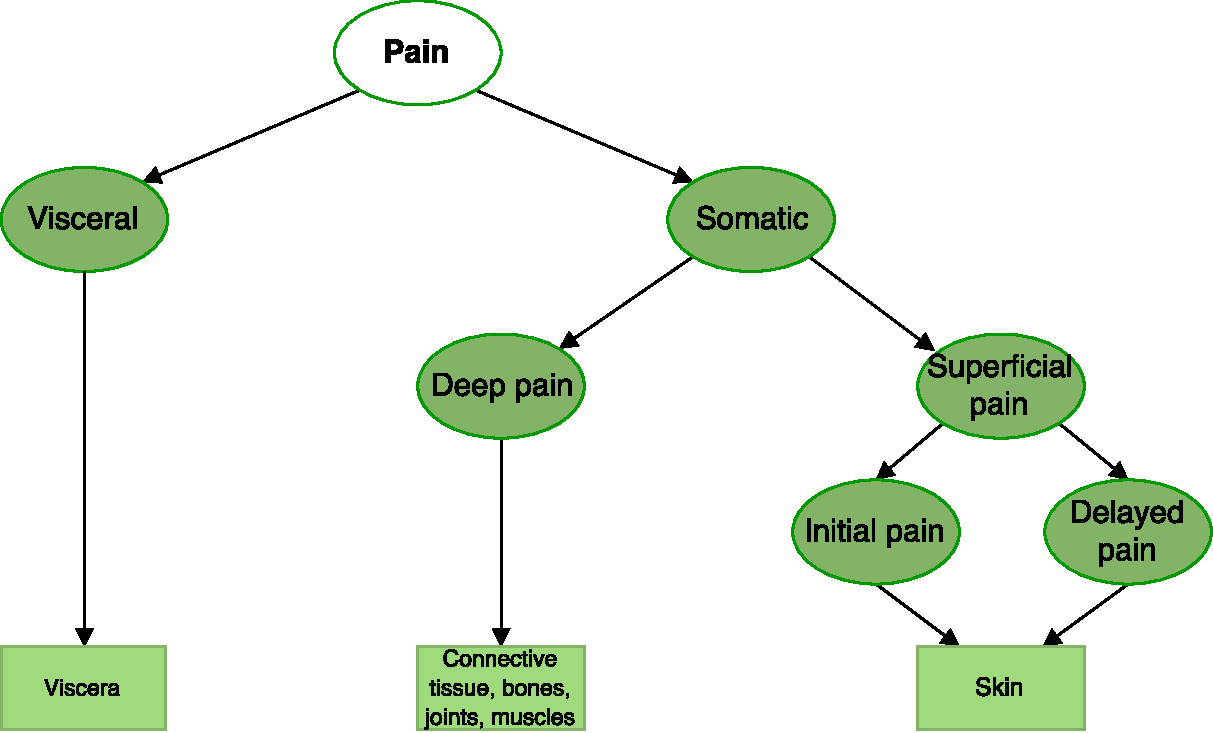
\includegraphics[width=0.75\textwidth]{figures/painpic}
\caption{Model of pain qualities. Ovals with green background  represent qualities of pain. The rectangles show where the pain originates. Edited \citep{Schmidt2013}.}
\label{fig:qualities}
\end{figure}

\noindent
Pain can be divided into two qualities; visceral and somatic pain. Examples of visceral pain include pain associated with gallstone and appendicitis. This pain can be characterised as a dull or diffuse feeling. Somatic pain is subdivided into superficial pain and deep pain. If the pain derives from the skin it is superficial pain, which furthermore is divided into initial pain and delayed pain. The initial pain is the first pain that is received, and characterised as sharp and localizable. The delayed pain, also known as the second pain, is a dull or burning pain that occur after a half to one second. This pain is more difficult to localise than the initial pain and lasts longer.\citep{Schmidt1989, Schmidt2013}
The other type of somatic pain is deep pain, which is associated with pain from the muscles, bones, joints and connective tissue. This pain is described as a dull pain and it radiates into the surrounding tissue, which makes the exact pain area hard to point out.\citep{Schmidt1989, Schmidt2013}




\section{Patellofemoral pain syndrome}
PFPS is a painful musculoskeletal condition \citep{Maclachlan2017, Smith2015}, which presents pain behind or around the patella. The patellofemoral pain (PFP) is often known as anterior knee pain and runner’s knee. The pain is often described as diffuse knee pain, which is provoked by patellofemoral loaded activities like climbing stairs, running on hard or slanted surfaces, hiking, squatting or just prolonged sitting in the same position.\citep{Crossley2016, Crossley2015, Smith2015, Boudreau2017} The pain is therefore not caused by previous trauma \citep{Crossley2016}.
Knee pain is not the only symptom of PFPS, the patient often complain about knee stiffness, patellofemoral crepitus, swelling knee and having trouble with common daily activities \citep{Martini2012, Crossley2016}. The patients may limit or stop the physical activity because of the pain, and that can lead to weight gain \citep{Petersen2013, Crossley2016}.\newline
\noindent
Physiologically PFPS is associated with incorrect movement of the patellar, that occurs when the patella moves outside of its ordinary track, which for instance can be movement in lateral direction instead of movement in superior-inferior direction.\citep{Martini2012} \newline
\noindent
PFP is mostly prevalent in adolescents and younger adults who are physically active, but it can affect people of all ages and activity levels \citep{Crossley2016, Maclachlan2017, Crossley2015}. Additionally,  females are affected about more than twice as often as males \citep{Petersen2013}. Furthermore, the PFPS can persist for up to 20 years and lead to osteoarthritis \citep{Petersen2013, Crossley2016}.\newline
\noindent
Despite the fact that patients feel pain in the knee, there is not any structural changes in the knee such as significant chondral damage or increased Q-angle \citep{Petersen2013}. The Q-angle, also known as the quadriceps angle, is the angle between a line that follows the longitudinal axis of femur, and a line that follows a line from the tibial tubercle through the center of patella \citep{Dahab2011}. \newline
\noindent
There is no definitive clinical test to diagnose PFP, but there is a test to elicit the knee pain by during a squatting manoeuvre. The PFP is evident in 80 \% of people who are tested positive in this test.\citep{Crossley2016, Crossley2015} Therefore the diagnosis PFPS is often based on exclusion \citep{Petersen2013}. After the diagnosis  evidence based treatments can reduce pain and improve function that allows patients to maintain physical activity \citep{Crossley2015}.
The aetiology of PFPS still remains unclear \citep{Smith2015}. \newpage


***
\noindent
Since the aetiology of PFPS still remains unclear \citep{Smith2015}, it is hard to place this type of pain in addition to nociceptive and neuropathic pain. But PFPS can be classified as deep pain and acute or chronic pain. Since the symptom duration often is longer than six month it is described as a chronic deep pain. ****

\section{Identify and interpret pain}
There are many ways to identify and interpret pain. To identify pain and find some physical damage that causes the pain can objective methods be used. Subjective methods is used to interpret pain for collecting knowledge of the individual's pain intensity, behavior and how it is experienced.\citep{Younger2009}

\subsection{Identify cause of pain}
An objective pain measurement is often used when an individual experiences knee pain where a clinical examination of the knee can occur. This examination involves i.a. provocative tests, such as anterior and posterior drawer test, Lachman’s test and pivot test that examines the integrity of the ACL and PCL. Furthermore is McMurray test which test for meniscal tear.\citep{Ghosh2010} Illustrations of the tests are shown in figure \ref{fig:kneetest}.

\begin{figure} [H]
\centering
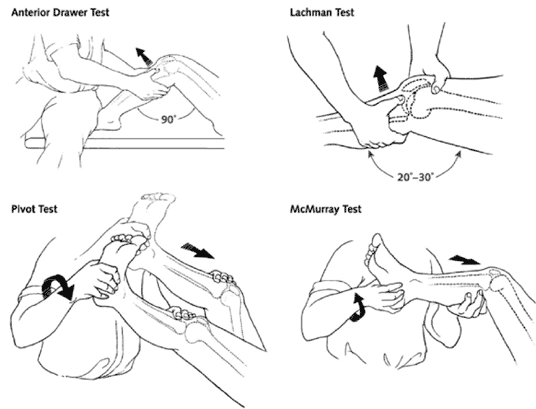
\includegraphics[width=0.78\textwidth]{figures/kneetest}
\caption{Clinical examination with provocative tests; Anterior Drawer Test, Lachman Test, Pivot Test and McMurray Test.\citep{Ghosh2010}}
\label{fig:kneetest}
\end{figure}


\noindent
In addition to clinical tests there is some paraclinical tests such as X-ray and MRI, but PFPS does not show any structural changes in the knee, like increased Q-angle or significant chondral damage \citep{Petersen2013}, which makes it difficult for healthcare personnel to treat the individuals. 

\subsection{Pain interpretation}
Pain is experienced and perceived subjectively \citep{IASP2012, Younger2009} and is dependent on personality and character \citep{Schmidt2013}, which is why it is important to measure the pain from the individual’s perspective.
 
\noindent
One of the most commonly method used to measure pain intensity is Visual Analogue Scale (VAS) \citep{Valente2011}. VAS is often used in clinical and research settings, where the individuals mark their pain on a scale from no-pain to the worst pain they can imagine.\citep{Haefeli2005} A illustration of a VAS is shown in figure \ref{fig:VAS}.

\begin{figure} [H]
\centering
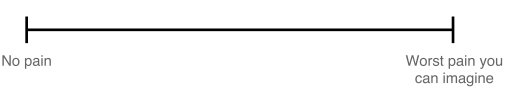
\includegraphics[width=0.8\textwidth]{figures/VAS}
\caption{Visual Analogue Scale (VAS). Edited from \citep{Haefeli2005}.}
\label{fig:VAS}
\end{figure}

\noindent
Additionally to mark pain on a scale is questionnaires used to define individual's pain. An example on a questionnaire is Knee injury and Osteoarthritis Outcome Score (KOOS), which contains questions about symptoms, stiffness, pain, function daily living, function, sports and recreational activities and quality of life. When the individuals fill the scheme a score between zero and one hundred is achieved. A score at zero represents extreme knee problems, whereas a score at one hundred represents no knee problems.\citep{Roos2003} The questionnaire can be seen in Appendix \ref{app:KOOS}. 
\noindent 
Since PFPS is described as a diffuse pain, where individuals indicate their pain by 'placing both hands over their knees', is it hard for individuals to precise communicate their pain. Thereby pain mapping is a method for individuals to better indicate and communicate their pain. 

\subsubsection{Pain mapping}
Pain mapping is a technique, that Harold Palmer introduced in 1949 \citep{Grunnesjo2006}, which is used to transfer a patient’s perceived pain into an objective graph or map by drawing the pain area. Pain drawings can be made by the patients who draw their pain areas on a body outline. Pain drawing can also be made by observers who observe the patients and then draw from the signs the patients are showing. An example of a body outline is shown in figure \ref{fig:painmap}. Sometimes a questionnaire is added to the pain drawings to get a more detailed overview of the pain to determine parameters associated with the pain. These parameters can also be useful in determining the source of the pain.\citep{Schott2010}

\begin{figure} [H]
\centering
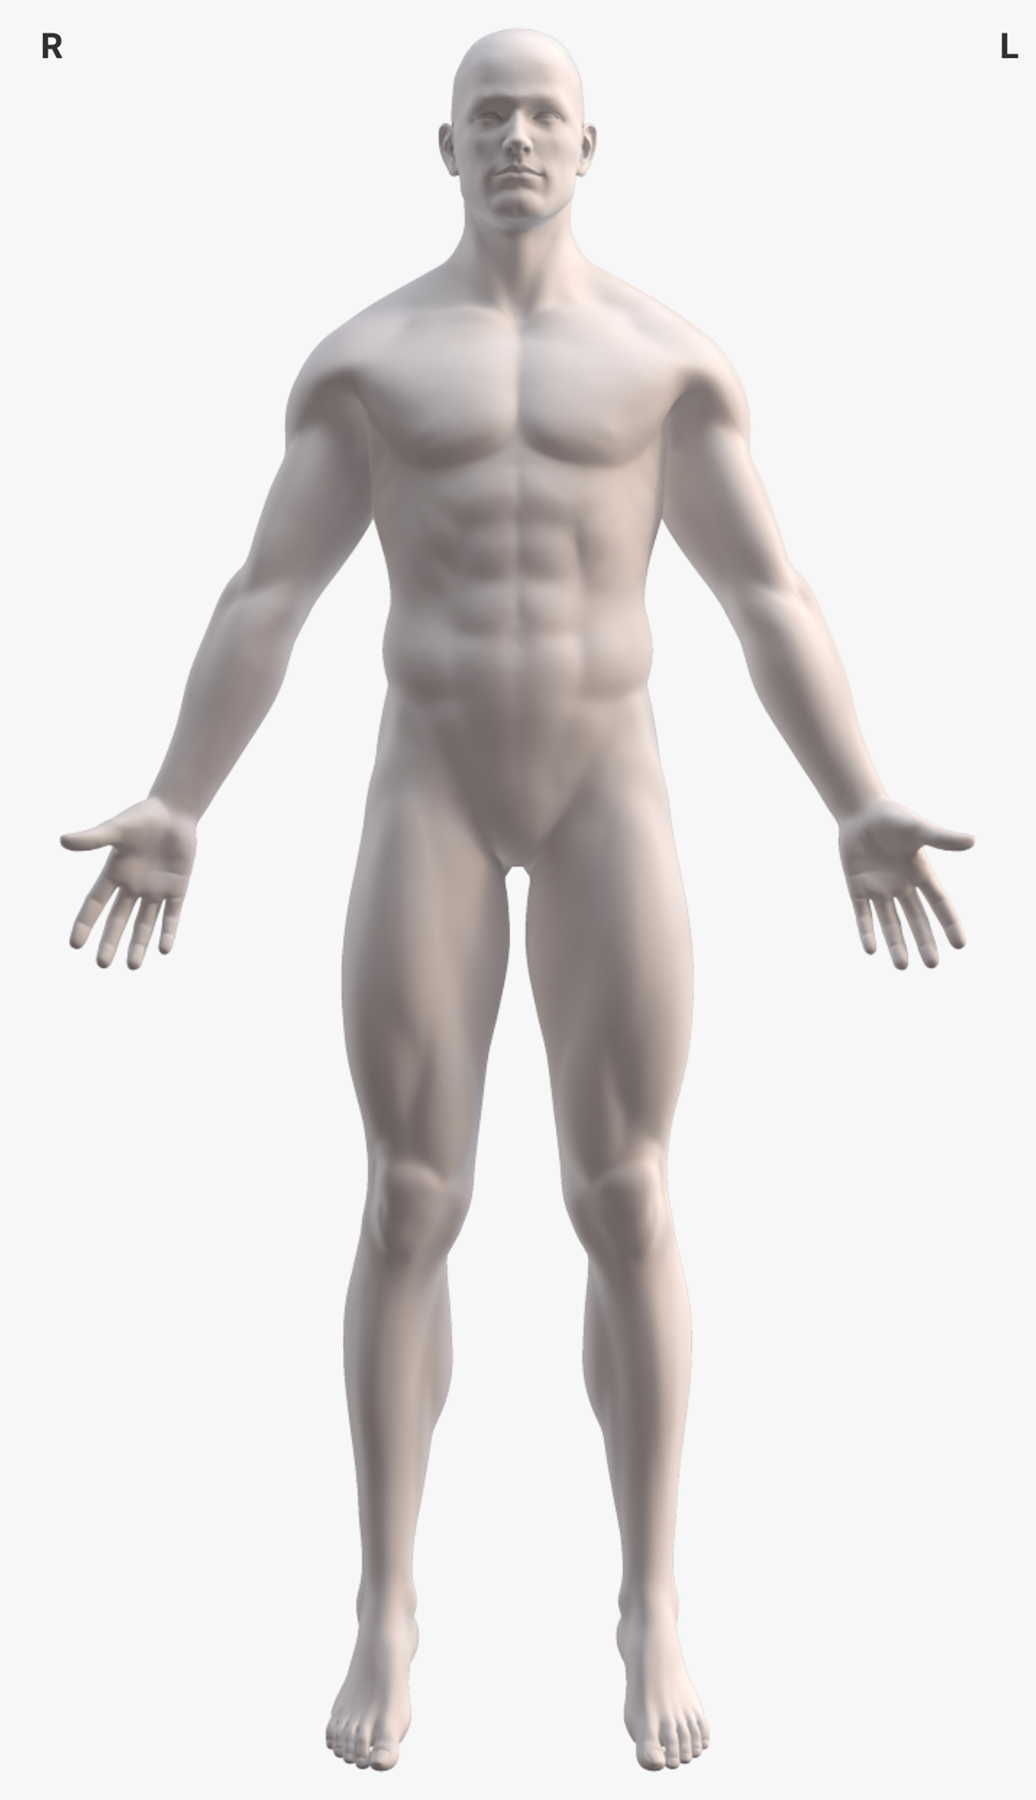
\includegraphics[width=0.3\textwidth]{figures/painmap}
\caption{The figure illustrates an anterior body outline for pain drawing. The figure is a screenshot from the application Navigate Pain.}
\label{fig:painmap}
\end{figure}

\noindent
Pain mapping are commonly used in clinical practice \citep{Schott2010}, and can be useful for patients when they try to describe their pain. Pain maps may also be helpful in diagnosing patients and follow-ups during or after treatment to get an indicator of the patient’s response to the treatment.\citep{Boudreau2016}
According to \citeauthor{Schott2010} there are some issues with the graphical representations of pain, some of which are problems with drawing a three-dimensional feeling of pain on a two-dimensional surface, and distinguishing between internal and external perceived pain on a map.\citep{Schott2010}

\section{Knee regions}

Patients with PFPS often describe the knee pain as a diffuse pain, and when looking at pain drawing samples from multiple patients it is also evident that there is a high variability in the distribution of pain patterns across different areas of the knee.

\noindent
To distinguish between different pain areas, the knee can be divided into various regions as seen in figure \ref{fig:atlas}, where the division of the left and right anterior knees are illustrated. 

\begin{figure} [H] 
\centering
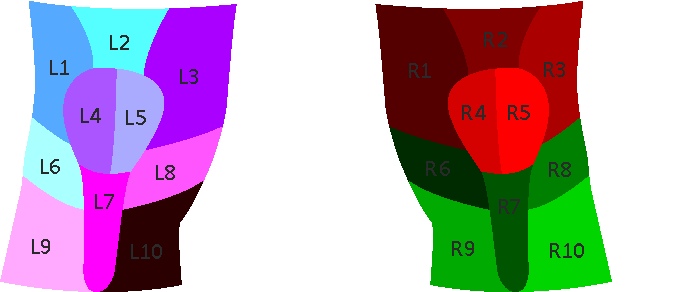
\includegraphics[width=0.6\textwidth]{figures/atlas}
\caption{The regions of the left and right knees, where each knee is split into ten regions.}
\label{fig:atlas}
\end{figure}

\noindent
The divisions is inspired by Photographic Knee Pain Map (PKPM) which is designed to categories location of knee pain, diagnostic and research purposes. PKPM represent both knees that makes it possible to identify unilateral and bilateral pain.\citep{Elson2010}

\noindent
The regions are based on the anatomic structures according to the areas where individuals often indicate pain.
There is ten regions, where region 1 and 3 represent the superior lateral and superior medial areas for patella. Region 2 refers to quadriceps tendon. The patella is divided into lateral and medial regions, which are region 4 and 5. Region 6 and 8 are lateral and medial joint line areas. Patella tendor is region 7 and the two last regions, 9 and 10, are tibia lateral and medial.\citep{Elson2010}

\newpage
